\chapter{Architektur}
\label{cha:architektur}

Die Software-Architektur unserer App musste sich in erster Linie den Besonderheiten des Android-Systems anpassen. Dazu wurden neben den Java Paketen hauptsächlich die spezifischen Android Bibliotheken benutzt.

Um die funktionalen Anforderungen zu erfüllen, wurde ein Datenmodell zur Speicherung während der Laufzeit sowie zur persistenten Speicherung benötigt. Die wichtigsten Datenobjekte bei dem Quartett-Spiel sind \emph{Deck} sowie \emph{Card}, wobei ein Deck aus mehreren Karten und eine Karte aus mehreren Bildern sowie Attributwerten besteht.

Eine zentrale funktionale Anforderung ist die Anbindung an einen REST-Server, von dem neue Kartendecks geladen werden können. Die Architektur benötigt also ein Modul, das HTTP-Anfragen senden, textbasierte Daten empfangen und diese in das interne Datenformat umwandeln kann.

Die eben genannten Aspekte werden im Folgenden näher erläutert.

\section{Besonderheiten in Android}
\label{sec:besonderheiten_android}

Eine Android-App setzt sich aus einer oder mehreren \emph{Activities} zusammen. Außerdem ist der App eine \emph{AndroidManifest.xml} Datei zugeordnet, die die enthaltenen Activities deklariert und in eine hierarchische Beziehung zueinander stellt. Activities werden als Java-Klassen implementiert, die von der Klasse \emph{Activity} aus der Android Bibliothek ableitet. Den Einstiegspunkt in die App bildet die \emph{MainActivity}.

\subsection{Activity Lifecycle}
\label{sec:activity_lifecycle}
\begin{figure}[ht]
\centering
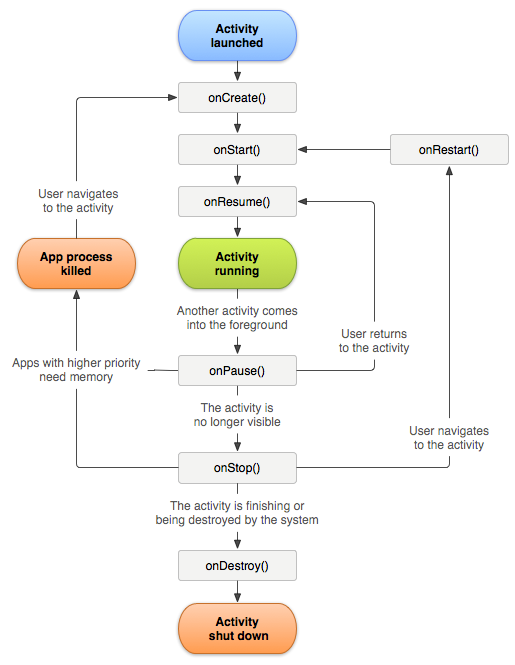
\includegraphics[width=\textwidth]{../img/ActivityLifecycle.png}
\caption{Activity Lifecycle}
\label{fig:activitylifecycle}
\end{figure}

Das Speichermanagement wird vom Android-System im Hintergrund geleistet. Aus Speicherplatz- und Energieeffizienzgründen auf mobilen Geräten haben Activities einen sogenannten Lifecycle. Zu entsprechenden Zeitpunkten werden vom System die Methoden \emph{onCreate()}, \emph{onPause()}, \emph{onStop()} usw. aufgerufen (siehe Abbildung \ref{fig:activitylifecycle}). In diese Methoden wird vom Anwendungsprogrammierer Code eingefügt, hierdurch kann er bei auftreten der entsprechenden Zustandsübergänge gewünschtes Verhalten implementieren und so z.B. aktuelle Daten vor dem Schließen der Anwendung persistieren.

\subsection{Layouts und Views}

Um eine GUI anzuzeigen benötigt die Activity ein Layout. Das Layout wird i.d.R. in \emph{onCreate()} mit dem API \emph{setContentView()} gesetzt. Layouts werden in XML Resourcen spezifiziert. Ein Layout enthält hierarchisch angeordnete \emph{Views} (dazu gehören Buttons, TextViews, Checkboxes, ProgressBars, ImageViews usw.). Views erhalten Attribute, die ihre Größe und Position im Layout und ihr Erscheinungsbild festlegen. Außerdem können sie ID-Attribut enthalten, mit dem in der Activity auf sie zugegriffen werden kann.

Die Methode \emph{findViewById()} liefert eine Referenz auf die entsprechende View-Instanz. Diese kann nun programmatisch verändert werden. Views implementieren das Observer-Pattern und ermöglichen damit ereignis-orientierte Programmierung. Die Klasse \emph{View} (bzw. davon abgeleitete Klassen) nehmen  Listener-Objekte entgegen, welche Methoden enthalten, die bei dem entsprechenden Ereignis aufgerufen werden.

\subsection{Kommunikation zwischen Activities}

Zu einem Zeitpunkt ist i.d.R. nur eine Activity aktiv. Beim Wechsel von einer Activity zu einer anderen müssen jedoch Informationen übergeben werden können. Der Wechsel erfolgt zentral durch die Methode\emph{startActivity()}. Sie erhält ein \emph{Intent}-Objekt, welches die Informationen in serialisierter Form enthält. Zu übergebende Objekte müssen hierzu das \emph{Serializable}- oder \emph{Parcelable}-Interface implementieren.

\subsection{Activities in FancyQuartett}
\label{sec:activities_in_fancyquartett}
\begin{figure}[ht]
    \centering
    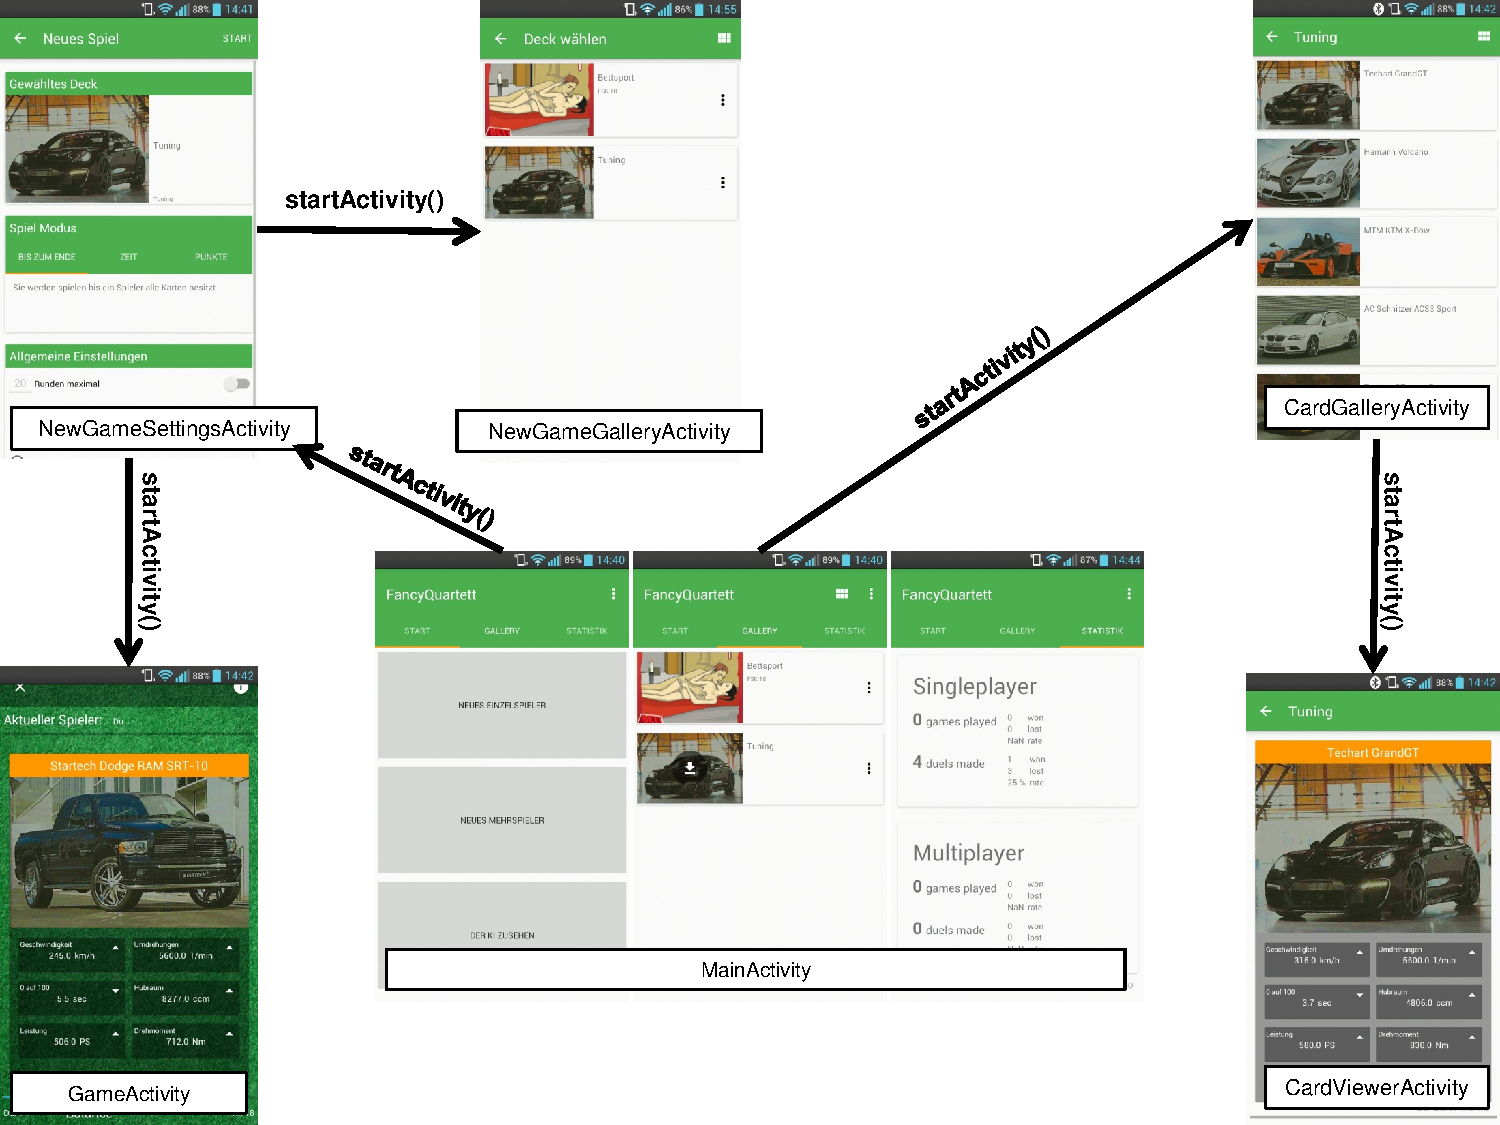
\includegraphics[width=\textwidth]{../img/Activities.pdf}
    \caption{Die Activities in FancyQuartett}
    \label{fig:activities_in_fancyquartett}
\end{figure}

Insgesamt werden 8 Activities verwendet, deren Struktur Abbildung \ref{fig:activities_in_fancyquartett} zeigt, welche hier kurz erläutert werden.

Die \emph{MainActivity} besteht aus 3 Fragmenten. Fragmente sind \emph{Sub-Activities}, die in eine Activity eingebettet sind und haben ihren jeweils eigenen Lifecycle. Sie können beispielsweise in einem sogenannten \emph{ViewPager} als Tabs verwendet werden.

Das erste Fragment dient als GUI zum starten eines Spiels. Startet der Benutzer ein neues Spiel, wird zur \emph{NewGameSettingsActivity} gewechselt. Diese dient zum wählen eines Decks und der Spieleinstellungen. Zum wählen eines Decks wird die \emph{NewGameGalleryActivity} gestartet, die alle verfügbaren Decks (sowohl offline als auch online) anzeigt. Nach dem Klick auf Start wird zur \emph{GameActivity} gewechselt. Diese stellt die aktuelle Karte dar und instanziiert die Klasse \emph{GameEngine}, welche die Ausführung der Spiellogik übernimmt.

Das zweite Fragment stellt die Deck-Gallerie dar. Bei der Auswahl eines Decks wird die \emph{CardActivity} gestartet, die alle Karten des Decks in einer \emph{ListView} anzeigt. Wird eine Karte ausgewählt wird die \emph{CardViewerActivity} gestartet, die die Karte mit ihren Bildern und Attributwerten in einem \emph{ViewPager} anzeigt. Durch \emph{Swipen} nach links bzw. nach rechts kann zur vorherigen bzw. nächsten Karte des Decks navigiert werden.

Das dritte Fragment zeigt eine Statistik an und bietet keine Interaktionsmöglichkeiten.

\section{Datenmodell}
\label{sec:datenmodell}

\begin{figure}[ht]
    \centering
    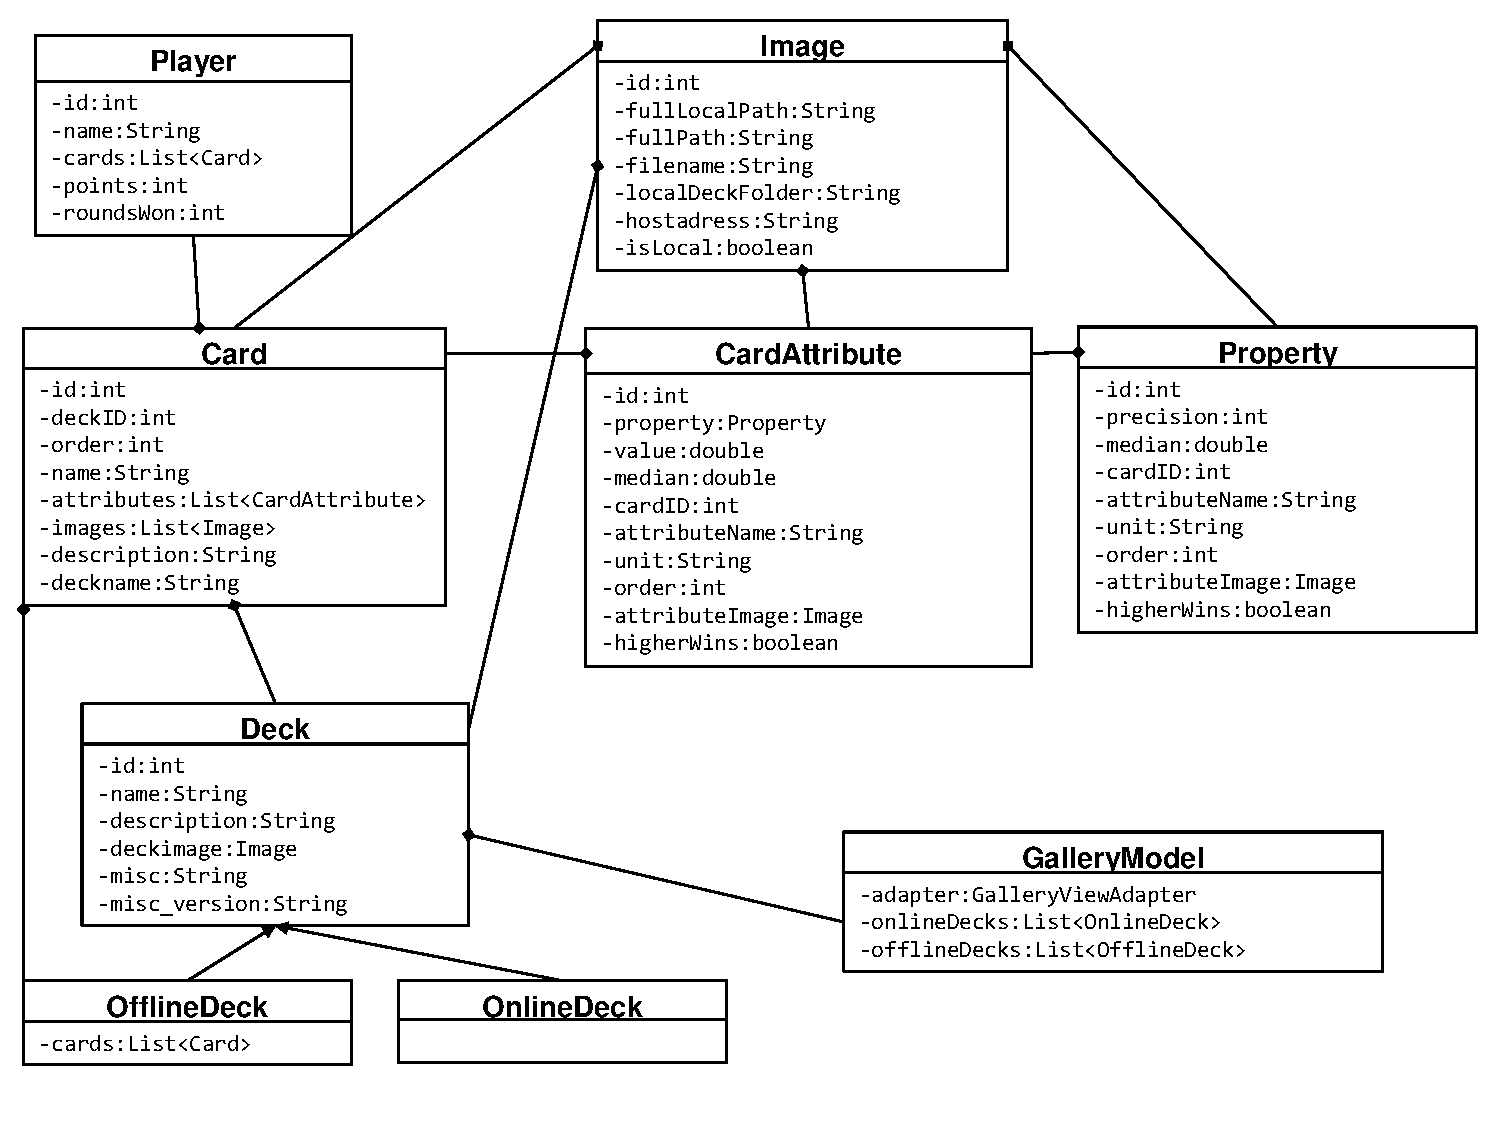
\includegraphics[width=\textwidth]{../img/Datenmodell.pdf}
    \caption{Datenmodell von FancyQuartett}
    \label{fig:datenmodell}
\end{figure}

Abbildung \ref{fig:datenmodell} zeigt die Realisierung der Datenbasis von FancyQuartett. In dieser Form werden die Daten zur Laufzeit gehalten.

Die persistente Speicherung erfolgt auf dem Dateisystem. Android weist jeder App einen Bereich im Dateisystem zu. Dort wird mittels der Klasse \emph{DeckDownloader} für jedes heruntergeladene Deck einen Ordner angelegt, in dem eine JSON Datei und die zu den Karten gehörenden Bilder gespeichert werden. \emph{DeckDownloader} erbt von der Klasse \emph{AsyncTask}. Das ermöglicht es, die Ein-/Ausgabe-Operationen in einem separaten Thread (asynchron) auszuführen, um die GUI nicht zu blockieren.

\section{Netzwerkfunktionen}
\label{sec:netzwerkfunktionen}

Für das Laden von Decks über das Netzwerk wurde ein Server mit einer REST-API zur Verfügung gestellt, der Daten im JSON-Format sendet. Von diesem konnten folgende Ressourcen abgefragt werden:
\begin{itemize}
    \item \textbf{/decks} liefert ein Array aus Objects. Die Anzahl der Objects entpricht den verfügbaren Decks. Die Objects enthalten jeweils die für ein Deck relevanten Informationen, die den Attributen im obigen Klassendiagramm in Abbildung \ref{fig:datenmodell} entsprechen.
    \item \textbf{/decks/<ID>} liefert das Deck-Object mit der entprechenden ID.
    \item \textbf{/decks/<ID>/cards} liefert ein Array aus Objects, die jeweils die ID und den Namen einer Karte enthalten.
    \item \textbf{/decks/<ID>/cards/<ID>} liefert das Card-Object mit der entsprechenden ID. Die Attribute in diesem Object nicht enthalten.
    \item \textbf{/decks/<ID>/cards/<ID>/attributes} liefert ein Array aus Objects, die jeweils die für ein Attribut und dessen Wert relevanten Informationen enthalten.
\end{itemize}

Durch den Aufruf von \emph{openConnection()} auf den entsprechenden URLs wird ein \emph{HttpURLConnection}-Objekt zurückgegeben, auf welchem noch der erforderliche Authorization Header gesetzt werden muss um Zugang zur API zu erhalten. Die empfangenen Daten können bei einer erfolgreichen Anfrage aus einem \emph{InputStream} gelesen werden. 

Das Package \emph{org.json} macht das Handling der empfangenen JSON-Daten einfach. Es bringt für JSON spezifizierte Klassen und entsprechende Operationen mit. Ein \emph{JSONObject} bzw. \emph{JSONArray} kann direkt aus einem ASCII-String erstellt werden. Die Konvertierung in das interne Datenformat (siehe Abbildung \ref{fig:datenmodell}) erfolgt durch Aufrufe auf den Klassenkonstruktoren, wobei die Werte aus den JSON-Objekten übergeben werden.